%% ------------------------------------------------------------------------- %%
\chapter{Contexto Teórico}
\label{cap:conceitos}

Este capítulo apresenta, um a um, os conceitos mais elementares, 
e tenta harmonizar a terminologia empregada no decorrer do texto.


%% ------------------------------------------------------------------------- %%
\section{\Gls{tectonic}}
\index{\gls{tectonic}}
\label{sec:02_tectonica}

A \gls{tectonic} é \glsdesc*{tectonic}.

Uma das principais evidências das transformações geológicas do planeta 
são os \glspl{equake}. A figura \ref{f:global_epicenters} \citep{img_world_epicenters}
é um mapa global com a ocorrência geográfica dos tremores. Nele é possivel notar que 
os sismos não são distribuídos uniformemente pelo globo.

\begin{figure}[H]
   \centering
   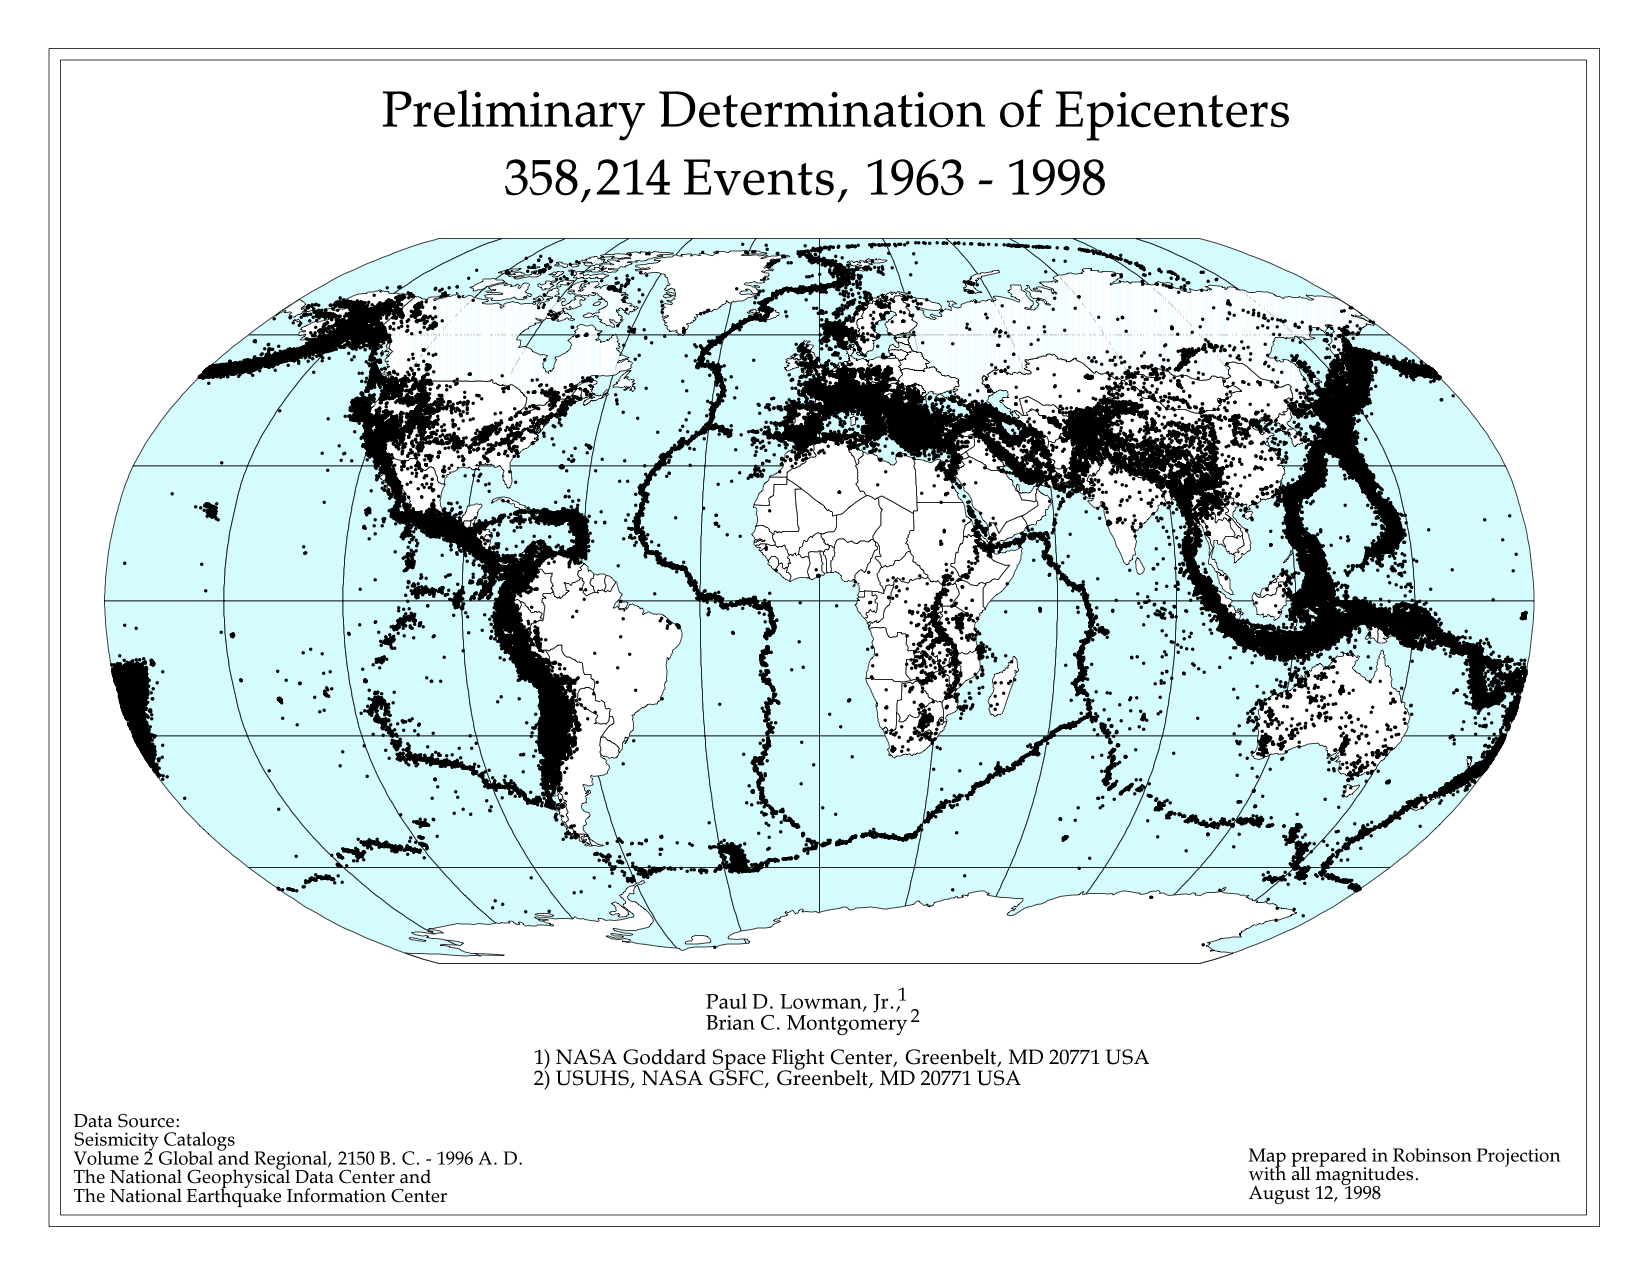
\includegraphics[width=0.80\textwidth]{global_pde_mag_all}
   \caption[Mapa Mundial de Epicentros 1963-1998]
   		   {Mapa Mundial de Epicentros 1963-1998\footnotemark} 
   \label{f:global_epicenters}
\end{figure} 
\footnotetext{\citet{img_world_epicenters}}
 
O padrão apresentado pela \gls{seismic_activity} global foi essencial 
para o desenvolvimento posterior da \gls*{tectonic_plate_theory}.

%% ------------------------------------------------------------------------- %%
\subsection{\Gls{tectonic_plate_theory}}
\index{\Gls{tectonic}!\Gls{tectonic_plate_theory}}
\label{sec:02_placas}

A \gls*{tectonic_plate_theory}, desenvolvida na segunda metade do século XX,
cartografava na superfície do globo as \glspl{litho_plate}.


\begin{figure}[H]
   \centering
   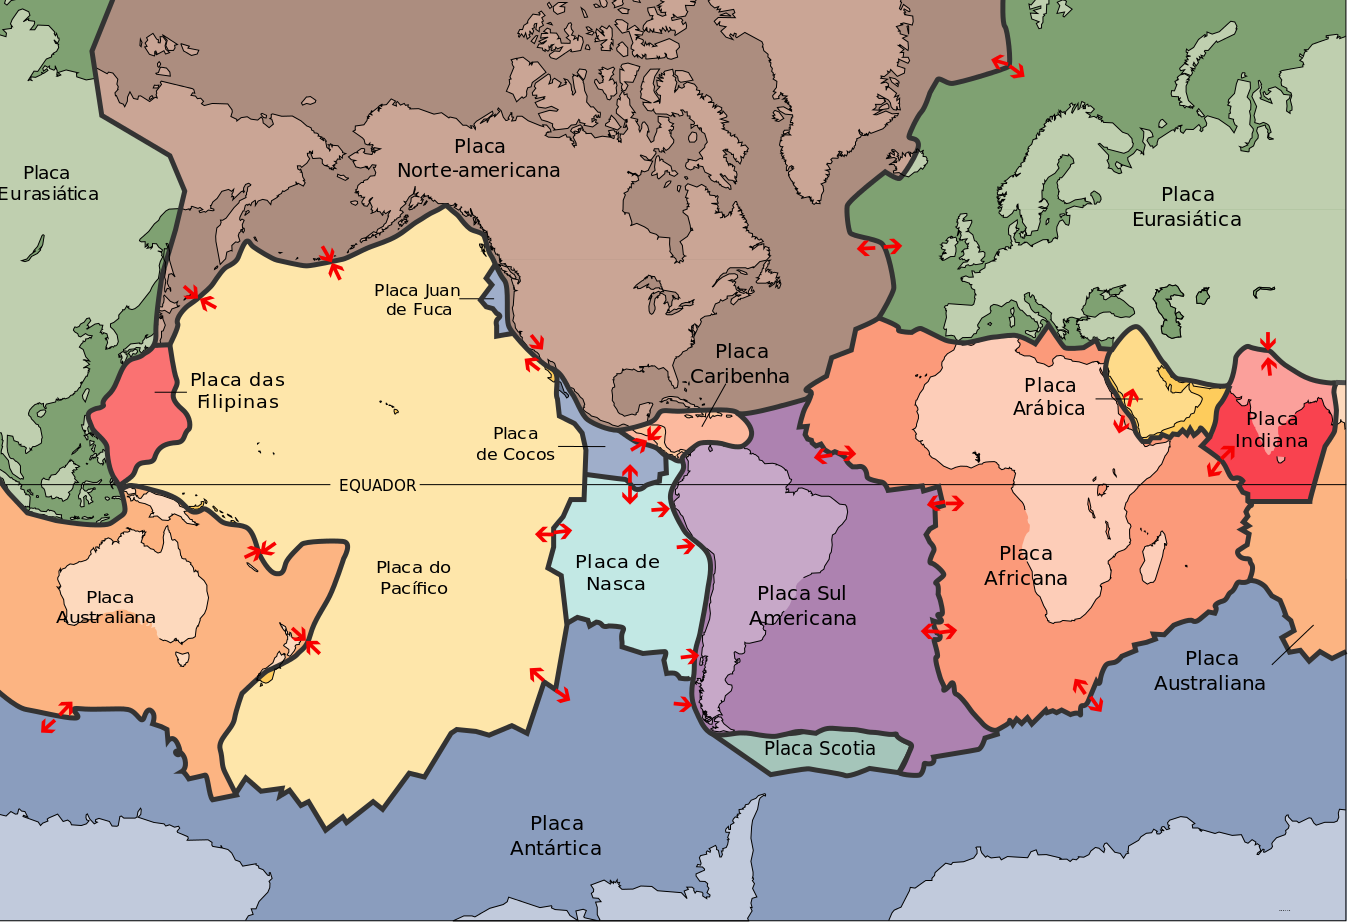
\includegraphics[width=0.80\textwidth]{litho_plates_overview}
   \caption[Cartografia das placas litosféricas]
   		   {Cartografia das placas litosféricas\footnotemark} 
   \label{f:plates_overview}
\end{figure} 
\footnotetext{\citet{img_plates_overview}}
 

As \glspl{litho_plate}, como pode ser visto na figura \ref{f:plates_overview},
e o conceito de \gls{astenosphere} (\glsdesc{astenosphere}) 
surgem para conformar uma teoria capaz de explicar
uma série de fenômenos tectônicos já observados e ainda não bem explicados na época
de seu desenvolvimento. 


%% ------------------------------------------------------------------------- %%
\subsubsection{Bordas}
\index{\Gls{tectonic_plate_theory}!bordas}
\label{sec:02_bordas}

Nas bordas das \glspl{litho_plate}, a tectônica é mais intensa, 
provocando uma enorme diversidade de fenômenos geológicos de acordo
com o tipo de interação, como ilustrado na figura \ref{f:plate_boundaries}.

\begin{figure}[H]
   \centering
   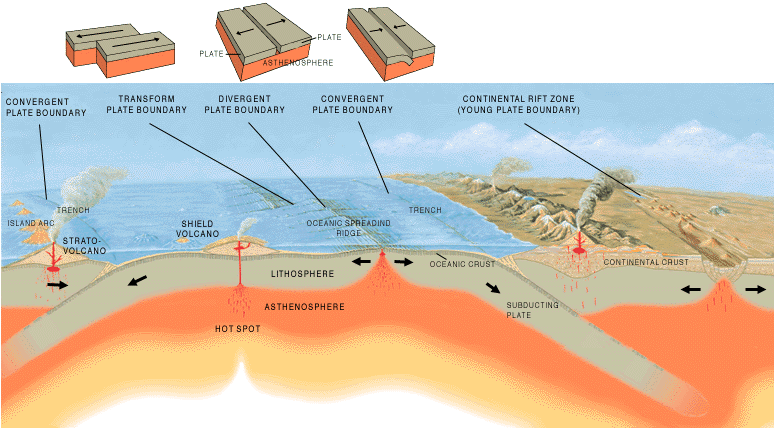
\includegraphics[width=0.80\textwidth]{plate_boundaries}
   \caption[Diferentes tipos de interações entre \glspl{litho_plate} em suas bordas]
   		   {Diferentes tipos de interações entre \glspl{litho_plate} em suas bordas\footnotemark} 
   \label{f:plate_boundaries}
\end{figure} 
\footnotetext{\citet{img_plate_boundaries}}
 
Na figura \ref{f:plate_boundaries} estão ilustrados os diferentes tipos de interação 
entre as \glspl{litho_plate} nas suas bordas, que causam, como já se sabe, a maior
parte dos \glspl{equake} e vulcanismo.

Só na borda das placas é liberada cerca de 95\% da quantidade total da energia 
disseminada na forma de \glspl{equake} no globo.

%% ------------------------------------------------------------------------- %%
\subsubsection{Interior}
\index{\Gls{tectonic_plate_theory}!interior}
\label{sec:02_interior}

A dificuldade maior é explicar, com maior detalhe, porque e como são liberados os outros 
5\% do total de energia em \glspl{equake}, mais raros, no interior das \glspl{litho_plate}.

Não há pleno consenso nem um modelo geral para a explicação do mecanismo de ocorrência dos
sismos no interior das placas, embora sejam conhecidas diversas zonas sísmicas em regiões no interior
de placas, como em Nova Madrid, nos Estados Unidos e também em locais da China e da Austrália para citar alguns.


%% ------------------------------------------------------------------------- %%
\subsection{Sismotectônica}
\index{\gls{tectonic}!\gls{seismotectonic}}
\label{sec:sismotectonica}

A \gls{seismotectonic} é \glsdesc*{seismotectonic}. 

Na prática consiste por um lado, num esforço de compreensão dos
processos geológicos através da observação dos tremores e analogamente, compreender os tremores através da observação
de processos geológicos mensuráveis.  

É fácil notar, portanto, a contribuição dessa disciplina para a análise de sismicidade.


\section{Sismicidade}
\index{sismicidade}
\label{sec:sismicidade}

A sismicidade é o estudo da ocorrência de dos tremores. Quando, onde, como, de que tamanho?!

É sabido que sismos menores são muito mais frequentes que os grandes tremores de terra
catastróficos.

Tremores de terra, abalos, \glspl{equake}, sismos são a ocorrência de
fenômenos geológicos de ruptura, instantânea, por certo mecanismo, de certa dimensão, na
crosta terrestre.


\subsection{Ocorrência}
\index{\gls{equake}!ocorrência}
\label{sec:ocorrencia}
 
Os tremores acontecem por uma ruptura geológica (figura \ref{f:rupture}) num tempo \gls{sym:t}, num lugar \gls{sym:r} e cada um
com seu tamanho \gls{sym:m}.

\begin{figure}[H]
   \centering
   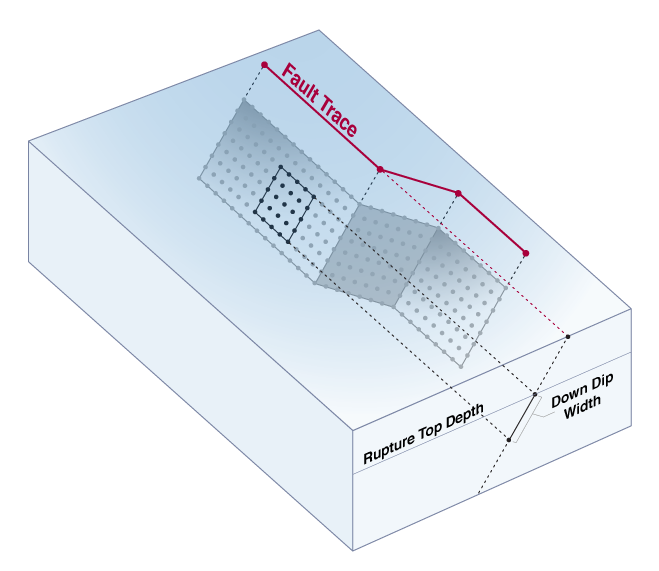
\includegraphics[width=0.50\textwidth]{rupture}
   \caption[Ilustração da área de ruptura em um falhamento geológico]
   		   {Ilustração da área de ruptura em um falhamento geológico\footnotemark} 
   \label{f:rupture}
\end{figure} 
\footnotetext{\citet{img_opensha_rupture}}
 

O local em que se iniciou a ruptura que deu origem ao tremor é um \gls{hypocenter},
enquanto sua projeção na superfície, desconsiderando-se a profundidade, é o \gls{epicenter}.


\subsubsection{Processo de Poisson}
\index{processo de Poisson}
\label{sec:processo_de_Poisson}

Definição do processo\ldots

Críticas\ldots

 
\subsection{Magnitude (da ruptura)}
\index{magnitude}
\label{sec:magnitude}

A magnitude de um tremor de terra é um valor medido numa escala que versa sobre a energia liberada pelo sismo, que é 
proporcional a área rompida e ao deslocamento geológico relativo entre as partes rompidas.

O desenvolvimento experimental de escalas de magnitude, para medir o tamanho dos tremores,
é marcado pelo trabalho do sismólogo Charges Richter \citep{richter_1935}.

Existem, entretanto, uma série de diferentes escalas de magnitude,
baseadas em diversos tipos de medidas. 

A escolha de qual usar fica a critério
de cada operador de sismógrafo e de cada rede sismográfica, que geralmente usam escalas diferentes
para avaliar a magnitude dos tremos, ou até mesmo divulgam mais de um tipo para
um mesmo evento.

As escalas são calibradas para fornecerem valores similares, de acordo com
o intervalo de utilidade para o qual foram desenvolvidas, mas apresentam diferenças consideráveis para um mesmo evento, 
podendo comprometer as análises estatísticas baseadas num catálogo cuja magnitude não tenha sido calculada de maneira uniforme.


\subsubsection{Magnitude Richter}
\index{magnitude!Richter}
\label{sec:magnitude_richter}

As escalas de magnitude mais comuns são as que derivam da definição de Richter \citep{richter_1935}
que se baseia na relação empírica entre o logarítmo da amplitude do registro das ondas sísmicas e a distância onde foram
registradas. Em 1935, Richter notou que:

\begin{equation}
	\gls{eqn:richter}
	\label{eq:richter}
\end{equation}
\glsdesc*{eqn:richter}.


A amplitude máxima de sua
escala foi definida pela amplitude máxima observada em um sismômetro Wood-Anderson, com período de 0.8s, registrando a 100km 
do tremor.

Na prática existem algumas incertezas e correções que deveriam ser feitas, principalmente pelo fato da escala estar intimamente 
relacionada a um determinado equipamento, hoje obsoleto, e porque que sismos locais (a menos de 100km) têm sua magnitude
melhor calculada usando frequencias mais altas que as registráveis pelo sismômetro da época.


Outras escalas foram desenvolvidas a partir da medida da amplitude máxima de determinadas fases 
(diferentes tipos de onda sísmica) e apresentam bons resultados para a maior parte dos sismos.
Não refletem, porém, com precisão, o tamanho dos maiores e mais destrutivos eventos, com magnitude acima de 7 ou 8.


\subsubsection{Magnitude de Momento Sísmico }
\index{magnitude!momento sísmico}
\label{sec:risco_sismico}

O evento de natureza sismológica ocorre num
instante \gls{sym:t} liberando uma certa quantidade de energia na forma de \glsdesc{sym:M_0}
\gls{sym:M_0} proporcional à \glsdesc{sym:M_W} \gls{sym:M_W} desse evento.

O \glsdesc{sym:M_0} é apresentado na equação \ref{eq:M_0}:

\begin{equation}
	\gls{eqn:M_0}
	\label{eq:M_0}
\end{equation}
\glsdesc*{eqn:M_0}.

O momento sísmico é estimado geralmente pela inversão duplamente acoplada de um tensor de momento aos registros em 
forma de onda do movimento do chão causado pelo terremoto. Ou, em casos de tremores muito bem registrados, ele pode
ser estimado a partir de algum modelo numérico para a ruptura.

A \glsdesc{sym:M_W} \gls{sym:M_W} \citep{hanks_1999} é baseada no 
logarítmo do \glsdesc{sym:M_0} \gls{sym:M_0}, e não se satura no caso de grandes eventos. 
Sua definição é dada pela equação \ref{eq:M_W} 

\begin{equation}
	\gls{eqn:M_W}
	\label{eq:M_W}
\end{equation}
\glsdesc*{eqn:M_W}.


\subsubsection{Intensidade Macrossísmica}
\index{instensidade macrossísmica}
\label{sec:intensidade}

A intensidade macrossísmica é uma escala para medir, não a energia proporcional
à ruptura que originou o tremor de terra, mas para retratar a percepção humana do
movimento do chão onde quer este tenha produzido seus efeitos.

Uma das mais difundidas é a escala Modificada de Mercalli \citep{richter_1958} apresentada em sua versão simplificada 
na tabela \ref{tab:mercalli}:

\begin{table}[H]
\begin{center}
\begin{scriptsize}
\noindent\begin{tabular}{c|c|p{12cm}}
\hline
Categoria  	& Sensação & Efeitos \\
\hline
I 			&	Imperceptível 	&	Não sentido. Apenas registado pelos sismógrafos.
\\II 		&	Muito fraco 	&	Sentido por um muito reduzido número de pessoas em 
								repouso, em especial pelas que habitam em andares
								elevados.
\\III 		&	Fraco 			&	Sentido por um pequeno número de pessoas. Bem sentido nos andares elevados.
\\IV 		&	Moderado 		&	Sentido dentro das habitações, podendo despertar do sono um pequeno número de pessoas. 
								Nota-se a vibração de
								portas e janelas e das loiças dentro dos armários.
\\V 		&	Forte 			&	Praticamente sentido por toda a população, fazendo acordar muita gente. 
								Há queda de alguns objectos menos estáveis e param os pêndulos dos relógios. 
								Abrem-se pequenas fendas nos estuques das paredes.
\\VI 		&	Bastante forte 	&	Provoca início de pânico nas populações. Produzem-se leves danos nas habitações, 
								caindo algumas chaminés. O mobiliário menos pesado é deslocado.
\\VII 		&	Muito forte 	&	Caem muitas chaminés. Há estragos limitados em edifícios de boa construção, 
								mas importantes e generalizados nas construções mais frágeis. 
								Facilmente perceptível pelos condutores de veículos automóveis em trânsito. 
								Desencadeia pânico geral nas populações.
\\VIII 		&	Ruinoso  		&	Danos acentuados em construções sólidas. Os edifícios de muito boa construção 
								sofrem alguns danos. Caem campanários e chaminés de fábricas.
\\IX 		&	Desastroso 		&	Desmoronamento de alguns edifícios. Há danos consideráveis em construções muito sólidas.
\\X 		&	Destruidor 		&	Abrem-se fendas no solo. Há cortes nas canalizações, torção nas vias de caminho 
								de ferro e empolamentos e fissuração nas estradas.
\\XI 		&	Catastrófico 	&	Destruição da quase totalidade dos edifícios, mesmo os mais sólidos. 
								Caem pontes, diques e barragens. Destruição das redes de canalização e das vias de comunicação. 
								Formam-se grandes fendas no terreno, acompanhadas de desligamento. Há grandes escorregamentos de terrenos.
\\XII 		&	Cataclismo 		&	Destruição total. Modificação da topografia. Nunca foi presenciado no período histórico. \\
\hline
\end{tabular}
\caption{Escala simplificada de intensidade sísmica, modificada em 1956 a partir da escala original de Giuseppe Mercalli de 1902}
\label{tab:mercalli}
\end{scriptsize}
\end{center}
\end{table}

Existem estudos \citep{bakun_1999} que propõem a inferência sobre o tamanho da ruptura, e sua
magnitude, a partir de observações macrossísmicas, ou dos efeitos relatados pela escala de intenside, georreferenciados.


%% ------------------------------------------------------------------------- %%
\subsection{Catálogos}
\index{catálogos}
\label{sec:catalogos}

Os catálogos podem ser vistos como uma coleção de parâmetros sobre os tremores. 
Podem ser classificados em três categorias \citep{woessner_catalog_2010} enumeradas a seguir:

\begin{itemize}\setlength{\itemsep}{0em}
	\item Pré-históricos: baseados na coleta de dados feitas por 
	geólogos estruturais em trincheiras ou campos de subsidência. Podem conter registros de tremores que ocorreram 
	há milhares de anos.
	\item Históricos: catálogos formados a partir de relatos históricos e inferência de valores de intensidade
	(seção \ref{sec:intensidade}), de análises de forma de onda com instrumentos antigos (registros em papel), eventualmente
	digitalizados.
	Cobrem o período das primeiras descrições humanas até os catálogos intrumentais.
	\item Instrumentais: são os catálogos de sismicidade definidos por dados produzidos por uma rede sismográfica bem estabelecida
	 gerando localizações continuamente (que começam a existir a partir de 1970).
\end{itemize} 

Os catálogos instrumentais são uma listagem onde se epera que encontrar para cada evento as seguintes informações:

\begin{itemize}\setlength{\itemsep}{0em}
	\item algum identificador,
	\item a localização (\gls{hypocenter}) do evento em algum sistema de referência (longitude, latitude, profundidade),
	\item o tempo de origem: data e hora com precisao de pelo menos décimos de segundo e
	\item uma ou várias informações de \glsdesc{sym:m}.
\end{itemize} 

Adicionalmente, embora não seja muito frequente, podem ser fornecidas informações adicionais obtidas pela análise das formas de
onda, como:

\begin{itemize}\setlength{\itemsep}{0em}
	\item incertezas sobre as magnitudes,
	\item incertezas sobre a localização (erro padrão, elipses de erro, cobertura dos sismogramas em diversas distâncias, cobertura
	dos sismogramas em vários ângulos azimutais, acurácia do modelo de velocidades utilizado, para enumerar alguns),
	\item intensidade máxima,
	\item intensidade no epicentro,
	\item número de, e as vezes as próprias, informações usadas para a determinação do hipocentro e hora de origem,
	\item sobre o mecanismo (alinhamento, mergulho e sentido do deslocamento na falha geológica) focal, entre outras.
\end{itemize} 

Mas é importante salientar \citep{woessner_catalog_2010} que cada um dos parâmetros determinados é fruto de uma série de decisões
e etapas de processamento.

Começam pela escolha dos sismômetros a serem instalados e onde para registrar as formas de onda. Sinais acima do nível de ruído
são associados à chegadas de fases quando registradas em mais de uma estação. 

A localização e o tempo de origem são
determinados juntando-se os tempos de chegadas das fases a um modelo de velocidade das ondas ao longo de camadas da crosta (ao
qual a localização é extremamente dependente). 

As magnitudes são computadas a partir das amplitudes e/ou da duração do sinal, dependendo profundamente da calibração dos
instrumentos.

\subsection{\glsdesc{mfd}}
\index{MFD}
\label{sec:mfd}

Observa-se que os sismos menores são muito mais frequêntes.
Entretanto, os maiores e mais raros são os que trazem a maior ameaça e os que causam as maiores perdas.

Uma análise conveniente seria explorar como se dá essa distribuição de magnitudes.

\subsubsection{\gls{mfd} de Gutenberg-Richter}
\index{Gutenberg-Richter MFD}
\label{sec:grmfd}

Gutenberg e Richter \citep{gr_1954} observaram empiricamente que a distribuição da frequência de ocorrência dos tremores e das
magnitudes seguiam uma deistribuição cuja versão clássica é apresentada na equação \ref{eq:gr_mfd} a seguir:

\begin{equation}
	\gls{eqn:gr_mfd}
	\label{eq:gr_mfd}
\end{equation}
\glsdesc*{eqn:gr_mfd}.

Com uma simples transformação de variáveis ($\alpha = 10^a$ e $\beta = b\ln{10}$), observa-se que o número de sismos que ocorrem 
com magnitudes dentro de um pequeno intervalo $[m, m+dm]$ tem distribuição exponencial:

\begin{equation}
	\begin{split}
		\gls{sym:N_m} &= 10^{\gls{sym:a} - \gls{sym:b}\gls{sym:m}} \\
					  &= \alpha e^{-\beta m}
	\end{split}
	\label{eq:gr_exp}
\end{equation}

A distribuição cumulativa, ou seja, o número de eventos com magnitude maior que um certo valor $m_{min}$ também segue uma
distribuição exponencial e é apresentada na equação \ref{eq:gr_cum}:

\begin{equation}
	\begin{split}
		N(m > m_{min}) &= \alpha \int\limits_{m_{min}}^{\infty}e^{-\beta m}\mathrm{d}m \\
					   &= \frac{\alpha}{\beta} e^{-\beta m} \\
					   &= \alpha_{cum} e^{-\beta m}
	\end{split}
	\label{eq:gr_cum}
\end{equation}
onde $\alpha_{cum} = \alpha / \beta $ é o valor cumulativo da atividade sísmica.


Entretanto, a distribuição clássica de \gls{gr} não impunha restrições sobre um limite inferior $m_{min}$ 
ou superior $m_{max}$ à validade da distribuição.


A figura \ref{f:mfd} apresenta um comparativo de algumas distribuições. Para ilustração, há também um histograma de um catálogo de
uma pequena região do norte do Chile, onde se pode observar que tanto a porção inferior (em torno de $m=5$), como a porção
posterior ($m > 7$) do histograma não seguem perfeitamente a distribuição. Há essencialmente duas zonas críticas em que é preciso
estar atento à física do problema:
(a) na parte inferior, muitos sismos de magnitude pequena não são registrados, pois não tem energia suficiente para sensibilizar
um conjunto razoável de estações que permita determinar suas localizações; (b) a parte superior, por sua vez, é crítica por se
acoplar diretamente aos limites físicos do tamanho da maior ruptura possível, relacionada diretamente ao limite de liberação de energia 
na forma de momento sísmico $M_0$.


\subsubsection{MFD Truncada}
\index{MFD Truncada}
\label{sec:TMFD}

Variações da distribuição clássica de \gls{gr} foram propostas em vista de melhor representar as MFD estudadas à partir de
catálogos de diversas regiões.

A equação \ref{eq:gr_max} versão incremental truncada com um limite superior $m_{max}$:

\begin{equation}
		\gls*{sym:N_m} = \frac{e^{-\beta m}}{1 -e^{-\beta m_{max}} }, m \leq m_{max}
	\label{eq:gr_max}
\end{equation}

Na equação \ref{eq:gr_dtr} versão incremental duplamente truncada com um limite inferior $m_{min}$ e superior $m_{max}$ :

\begin{equation}
		\gls*{sym:N_m} = \frac{e^{-\beta (m - m_{min})}}{1 -e^{-\beta (m_{max} - m_{min}) } } , m_{min} \leq m \leq m_{max}
	\label{eq:gr_dtr}
\end{equation}

A figura \ref{f:mfd} ilustra essas distribuições.

\subsubsection{MFD Limitada}
\index{MFD Limitada}
\label{sec:BMFD}

Outra possibilidade, é limitar suavemente a parte final da curva (ver figura \ref{f:mfd}). A equação \ref{eq:gr_bounded} apresenta
a distribuição:

\begin{equation}
		\gls*{sym:N_m} = \alpha [ e^{-\beta (m - m_{min})} - e^{-\beta (m_{max} - m_{min}) } ], m_{min} \leq m \leq m_{max}
	\label{eq:gr_bounded}
\end{equation}


\subsubsection{MFD com decaimento exponencial}
\index{MFD com decaimento exponencial}
\label{sec:KMFD}

Yan Kagan \citep{kagan_2002} propôs uma distribuição de magnitude mais adequada e acoplada à energia liberada pelos sismos, que
pode ser descrita como na equação \ref{eq:gr_tapered}:

\begin{equation}\ensuremath{
		\gls*{sym:N_m} = [\gls*{sym:beta_p} + \frac{m}{m_{min}}]
				m_{min}^{\gls*{sym:beta_p}}
				\gls*{sym:m_corner}^{-1 -\gls*{sym:beta_p}}
				e^{\frac{m_{min} - m}{\gls*{sym:m_corner}}}, 
				m_{min} \leq m < \infty
		}
	\label{eq:gr_tapered}
\end{equation}
onde \glsdesc*{sym:beta_p} e \gls*{sym:m_corner} \glsdesc*{sym:m_corner}

A figura \ref{f:mfd} mostra a diferença entre algumas dessas distribuições

\begin{figure}[H]
   \centering
   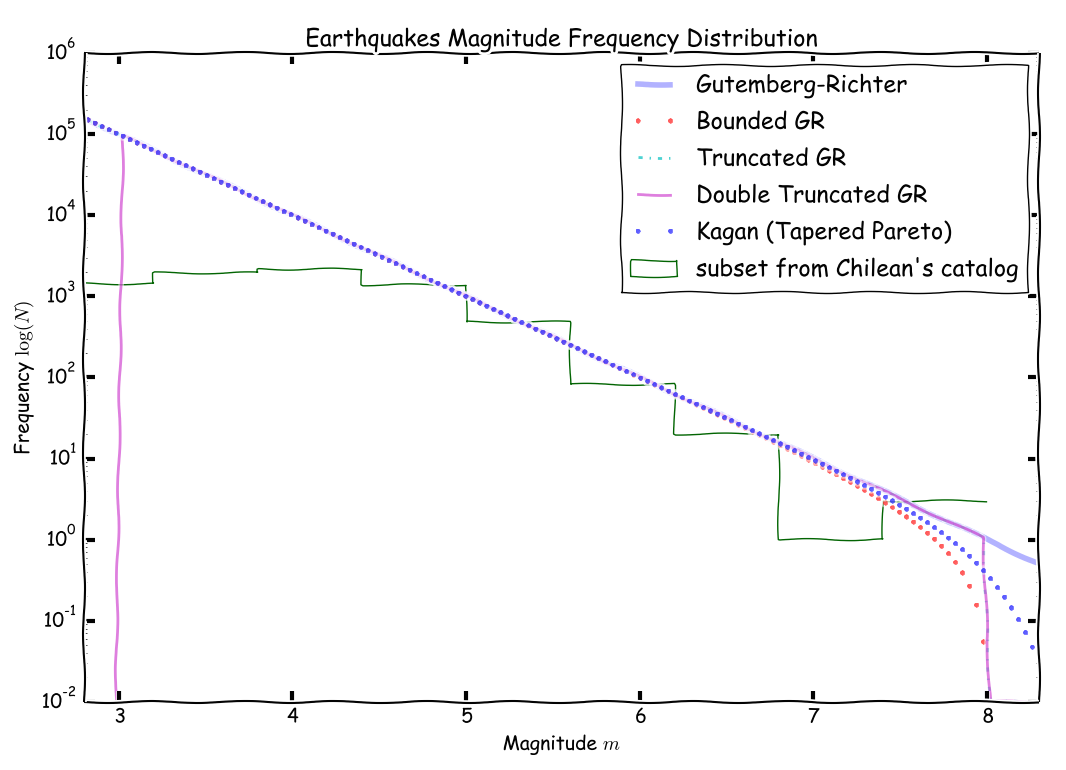
\includegraphics[width=0.95\textwidth]{mfd}
   \caption[Distribuições de frequência e magnitude]
   		   {Distribuições de frequência e magnitude} 
   \label{f:mfd}
\end{figure} 



\section{Taxa de Sismicidade}\index{área do
trabalho!fundamentos}
\label{sec:risco_sismico}


Texto texto texto texto texto texto texto texto texto texto texto texto texto
texto texto texto texto texto texto texto texto texto texto texto texto texto
texto texto texto texto texto texto texto texto texto texto texto texto texto


\subsubsection{Magnitude de Completude}\index{área do
trabalho!fundamentos}
\label{sec:risco_sismico}

A magnitude de completude\ldots 

texto texto texto texto texto texto texto texto texto texto texto texto texto


GRAFICO

FORMULA



\subsubsection{Valor-b}\index{área do
trabalho!fundamentos}
\label{sec:risco_sismico}


Texto texto texto texto texto texto texto texto texto texto texto texto texto
texto texto texto texto texto texto texto texto texto texto texto texto texto
texto texto texto texto texto texto texto texto texto texto texto texto texto


\subsubsection{Valor-a}\index{área do
trabalho!fundamentos}
\label{sec:risco_sismico}



Texto texto texto texto texto texto texto texto texto texto texto texto texto
texto texto texto texto texto texto texto texto texto texto texto texto texto
texto texto texto texto texto texto texto texto texto texto texto texto texto




\section{Risco Sísmico}\index{área do trabalho!fundamentos}
\label{sec:risco_sismico}

-> risk = ( hazard, 
			exposition, 
			vulnerability)


A redução do risco sísmico é um problema complexo, que envolve geralmente muitas pessoas, informações, decisões e ações.

A palavra risco, ao pé da letra, significa a exposição à possibilidade de injúria ou perda. E geralmente é usada como
sinônimo de ameaça. Na literatura acerca do tema risco, inclusive, as palavras são usadas com certa confusão.

No glossário da EERI (EERI Committee on Seismic Risk, 1984) a definição de risco sísmico é a probabilidade de que
perdas sociais ou econômicas aconteçam como decorrência de tremores superem limiares estabelecidos para determinado
local ou região durante um certo período de exposição.

A ameaça sísmica, por outro lado, é qualquer fenômeno físico (oscilação, falhamento) associado à terremotos que possam
produzir efeitos adversos às atividades humanas. Na prática são avaliados por dadas probabilidades de ocorrência.

Do que se pode deduzir que o risco sísmico é um produto da ameaça sísmica:

Seismic Risk = Seismic Hazard × Vulnerability × Value (1.1)

where vulnerability is the amount of damage induced by a given degree of hazard and expressed as a fraction of the value of the
damaged item under consideration. The × symbols in Eq. (1.1) do not represent multiplication, in fact, how seismic hazard,
vulnerability and value are to be combined depends on how they are expressed. Different ways to do so have been adopted in the
numerous procedures proposed in the literature (Dowrick, 2003) . To better understand the meaning of Eq. (1.1) it is worth
considering an example. One of the most complete risk assessment frameworks recently proposed is the PEER’s performance based
earthquake engineering methodology (Porter, 2003).

The principal outputs of PEER’s approach are system-level performance measures: probabilistic estimates of repair costs,
casualties, and loss-of-use duration (“dollars, deaths, and downtime”). The objective of the methodology is to estimate 
the frequency with which a particular performance metric will exceed various levels for a given design at a given
location. These can be used to create probability distributions of the
performance measures during any planning period of interest. From the frequency and probability distributions can be
extracted simple point performance metrics that are meaningful to facility stakeholders, such as an upper-bound economic loss during the owner-investor’s planning period. Figure 1.1 illustrates the PEER methodology. As it shows, PEER’s PBEE approach involves four stages: hazard analysis, structural analysis, damage analysis, and loss analysis. In the figure, the expression p[X|Y] refers to the probability density of X conditioned on knowledge of Y, and g[X|Y] refers to the occurrence frequency of X given Y (equivalent to the negative first derivative of the frequency with which X is exceeded, given Y). Eq. (1.2) frames the PEER methodology mathematically. Note that Figure 1.1 omits conditioning on D after the hazard analysis for brevity, but it is nonetheless implicit.

Eq. (1.2) can be considered as a specialization of Eq. (1.1): hazard maintains the same meaning, vulnerability is
expressed as the combination of the results of two stages, structural analysis and fragility analysis, and value is
evaluated by the loss analysis. Within this framework the × symbol represents convolution.
Seismic fragility and vulnerability of structures will be described in greater detail in the second part of this
dissertation, while this part is focused on seismic hazard assessment and on defining input for structural analysis in
terms of accelerograms.
For design or risk assessment purposes the assessment of seismic hazard consists of the following basic steps:
− definition of the nature and location of earthquake sources
− magnitude-frequency relationships for the sources
− attenuation of ground motion with distance from source
− determination of ground motions at the site having the required probability
of exceedance.

Because seismic risk and hazard statements are essentially forecasts of future situations, they are inherently
uncertain. Seismic hazard assessment attempts to forecast the likely future seismic activity rate and strengths, based
on knowledge of the past and present, and significant uncertainties arise partly because the processes involved are not
fully understood and partly because relevant data are generally scarce and variable in quality. For reasonable
credibility considerable knowledge of both historical seismicity and geology need to be used, together with an 
appropriate analysis of uncertainties. Where available other geophysical or seismological knowledge, such as  crustal
strain studies, may also be helpful, particularly in evaluating regional seismic activity patterns.

The present chapter introduces the basis of the procedures that may be used to assess seismic hazard, giving particular
relevance to Probabilistic Seismic Hazard Analysis (PSHA). Some of the concepts described here (e.g. hazard curve,
xattenuation relationship, disaggregation) will be widely used in the following chapters of the present work.


\section{Ameaça Sísmica}\index{área do trabalho!fundamentos}
\label{sec:ameaca_sismica}

-> hazard = seismic sources, 
			rupture occurence, 
			ground motion prediction 

 
\subsection{Projeção da Ocorrência de Rupturas}
\index{área do trabalho!fundamentos}
\label{sec:fundamentos}

As projeções (\textit{forecasting}) são feitas para se estimar a ocorrência de futuros tremores,
principalmente dos maiores, com grandes chances de provocar perdas.

Nas de curto prazo, estimam-se os próximos tremores
numa escala de dias ou horas considerando uma taxa de sismicidade variável 
com o tempo como no caso dos pré e pós-abalos, ou de quando 
acontece um enxame sísmico, período de maior atividade numa região.
Sua principal aplicação são para tomada de decisões de curto período, 
como evacuação de edifícios.

Nas de longo prazo, foco desse texto, a principal consideração feita é de que a 
\gls{seismic_rate} não varie ao longo do tempo, servindo para estimar as acelerações 
provovadas por tremores que possam ocorrer,
mesmo que muito raramente, de grandes proporções. Suas aplicações fazem sentido quando
se deseja saber o nível de segurança e resistência estrutural que devem ser impostos 
às edificações em geral, ou o valor de um contrato de resseguro de plataformas de petroleo,
ou outros grandes investimentos industriais, como usinas nucleares.



Texto texto texto texto texto texto texto texto texto texto texto texto texto
texto texto texto texto texto texto texto texto texto texto texto texto texto
texto texto texto texto texto texto texto texto texto texto texto texto texto



\section{Análise Probabilistica de Ameaça Sísmica}\index{área do
trabalho!fundamentos}
\label{sec:psha}


cornell, mcguire ?!?


Texto texto texto texto texto texto texto texto texto texto texto texto texto
texto texto texto texto texto texto texto texto texto texto texto texto texto
texto texto texto texto texto texto texto texto texto texto texto texto texto



%% ------------------------------------------------------------------------- %%
\subsection{Caracterização de Fontes Sísmicas}
\index{ácido!nucléico}\index{nucleotídeos}
\label{sec:fontes}

cornell, mcguire ?!?


Texto texto texto texto texto texto texto texto texto texto texto texto texto
texto texto texto texto texto texto texto texto texto texto texto texto texto
texto texto texto texto texto texto texto texto texto texto texto texto texto



\subsubsection{Tipologia e Representação Geométrica}
\index{ácido!nucléico}\index{nucleotídeos}
\label{sec:fontes_tipologia}


\subsubsection{Falha Complexa}
\index{ácido!nucléico}\index{nucleotídeos}
\label{sec:fonte_falha_complexa}


Texto texto texto texto texto texto texto texto texto texto texto texto texto
texto texto texto texto texto texto texto texto texto texto texto texto texto
texto texto texto texto texto texto texto texto texto texto texto texto texto



\subsubsection{Falha Simples}
\index{ácido!nucléico}\index{nucleotídeos}
\label{sec:fonte_falha_complexa}



Texto texto texto texto texto texto texto texto texto texto texto texto texto
texto texto texto texto texto texto texto texto texto texto texto texto texto
texto texto texto texto texto texto texto texto texto texto texto texto texto



\subsubsection{Área}
\index{ácido!nucléico}\index{nucleotídeos}
\label{sec:fonte_falha_complexa}


Texto texto texto texto texto texto texto texto texto texto texto texto texto
texto texto texto texto texto texto texto texto texto texto texto texto texto
texto texto texto texto texto texto texto texto texto texto texto texto texto



\subsubsection{Pontos}
\index{ácido!nucléico}\index{nucleotídeos}
\label{sec:fonte_falha_complexa}


Texto texto texto texto texto texto texto texto texto texto texto texto texto
texto texto texto texto texto texto texto texto texto texto texto texto texto
texto texto texto texto texto texto texto texto texto texto texto texto texto



\subsection{Caracterização}
\index{ácido!nucléico}\index{nucleotídeos}
\label{sec:fontes}



Texto texto texto texto texto texto texto texto texto texto texto texto texto
texto texto texto texto texto texto texto texto texto texto texto texto texto
texto texto texto texto texto texto texto texto texto texto texto texto texto



\subsubsection{Ocorrência de Sismicidade}
\index{ácido!nucléico}\index{nucleotídeos}
\label{sec:fontes}


Texto texto texto texto texto texto texto texto texto texto texto texto texto
texto texto texto texto texto texto texto texto texto texto texto texto texto
texto texto texto texto texto texto texto texto texto texto texto texto texto


\subsubsection{Ocorrência de Sismicidade}
\index{ácido!nucléico}\index{nucleotídeos}
\label{sec:fontes}




Texto texto texto texto texto texto texto texto texto texto texto texto texto
texto texto texto texto texto texto texto texto texto texto texto texto texto
texto texto texto texto texto texto texto texto texto texto texto texto texto



\subsubsection{Caracterização de Fontes Sísmicas}
\index{ácido!nucléico}\index{nucleotídeos}
\label{sec:fontes}



Texto texto texto texto texto texto texto texto texto texto texto texto texto
texto texto texto texto texto texto texto texto texto texto texto texto texto
texto texto texto texto texto texto texto texto texto texto texto texto texto





%% ------------------------------------------------------------------------- %%
\subsection{Predição do Movimento do Chão} 
\index{Equação de Predição do Movimento do Chão}
\index{gmpe}
\label{sec:gmpe}


Texto texto texto texto texto texto texto texto texto texto texto texto texto
texto texto texto texto texto texto texto texto texto texto texto texto texto
texto texto texto texto texto texto texto texto texto texto texto texto texto



%% ------------------------------------------------------------------------- %%
\subsection{Cálculo da Curvas de Ameaça} 
\index{curvas ameaça}
\label{sec:curvas_de_ameaca}


Texto texto texto texto texto texto texto texto texto texto texto texto texto
texto texto texto texto texto texto texto texto texto texto texto texto texto
texto texto texto texto texto texto texto texto texto texto texto texto texto

